\documentclass[11pt]{article}

\usepackage[utf8]{inputenc}
\usepackage{graphicx}
\usepackage[italian]{babel}
\usepackage{amsmath}
\usepackage{amssymb}
\usepackage{hyperref}
\usepackage{listings}
\usepackage[margin=1.2in]{geometry}
\usepackage{enumitem}

\usepackage[autostyle=false]{csquotes}
\MakeOuterQuote{"} 

\usepackage{xcolor}

\lstdefinelanguage{sparql}{
  morecomment=[l][\color{purple}]{\#},
  morestring=[b][\color{blue}]\",
  morekeywords={SELECT,CONSTRUCT,DESCRIBE,ASK,WHERE,FROM,NAMED,PREFIX,BASE,OPTIONAL,FILTER,ORDER,BY,GRAPH,LIMIT,OFFSET,SERVICE,UNION,EXISTS,NOT,BINDINGS,MINUS,a},
  sensitive=true
}

\counterwithin*{section}{part}
\counterwithin*{footnote}{part}
\graphicspath{ {./img/} }

% lunedì        10:30-12:30 U14/T024 (U14/1)
% mercoledì     10:30-13:30 U14/T024 (U14/1)


% Semantic Web, tra Tecnologie e Open Data, Di Noia, De Virgilio, Di Sciascio, Donin, Apogeo, 2013
% Linked Data


\title{\textbf{Data Semantics}}
\author{}
\date{}

\begin{document}
\maketitle
\begin{abstract}
  La \textit{Data Semantcs} si occupa di comprendere il significato dei dati durante la scrittura di un programma.
  Nell'ambito dell'analisi è fondamentale nell'integrazione di più dataset e nella loro condivisione.
  Altra problematica che la \textit{Data Semantics} si pone di risolvere è l'organizzazione di dati non strutturati in modo da facilitarne l'analisi.
  
  Scopo del corso è costruire dei modelli per attribuire valore semantico ai dati, in modo tale da facilitarne la fruizione; si tenta inoltre di capire il ruolo della semantica nell'integrazione dei dataset.
  Le finalità del corso rientrano nell'ambito dei \textit{big data}, nella costruzione di \textit{knowledge graphs} (ovvero la costruzione di relazioni interne a un database) e la costruzione di sistemi di raccomandazione.
  Saranno inoltre analizzate alcune tecniche di \textit{natural language processing} per costruire rappresentazioni a partire dai dati. \newline
  Le esercitazioni si occuperanno di interrogare \textit{knowledge graphs} e integrare fonti di dati.

  L'esame orale sarà accompagnato da un progetto software (effettuato in gruppo di - circa - 3 persone), di cui sarà fatta una presentazione orale; in alternativa al progetto è possibile scrivere un articolo di approfondimento su una tematica a scelta.
  La preparazione dovrà essere ``ragionevolmente'' dettagliata su tutti gli argomenti, e particolarmente approfondita sull'argomento del progetto.
\end{abstract}

\newpage
\tableofcontents

\newpage
% titolo provvisorio
\part{Grafi di conoscenza ed introduzione ai concetti}
% non mi sembra molto coeso il discorso: correggere
Il termine "grafo di conoscenza" è stato coniato da Google per indicare uno strumento usato dal suo motore di ricerca per fornire informazioni aggiuntive durante le interrogazioni.
La struttura a grafo permette di essere processata facilmente da una macchina e allo stesso tempo garantisce un livello di astrazione soddisfacente; si possono anche effettuare query come in un database a grafo (Neo4j).
Il modello a grafo permette inoltre una facile integrazione di sorgenti diverse rendendo naturali collegamenti e relazioni.

Il web \textit{semantico} ha costruito linguaggi e strumenti, approvati dal W3C, per definire, interrogare e fare inferenza su grafi di conoscenza; tuttavia nel mondo reale questi strumenti non hanno largo utilizzo.
La costruzione di grafi di conoscenza è spesso effettuata a mano da una moltitudine di utenti (chiedendo recensioni tramite \textit{app}, ad esempio).
Internet produce enormi quantità di dati diversi tra di loro, usati spesso per altri fini: la semantica dei dati si occupa di integrare grandi quantità (\textit{data volume}) da diverse fonti di dati (\textit{data variety}).
Tali dati possono essere sfruttati nella costruzione di intelligenze artificiali, ovvero di programmi che eseguono task tipicamente umani con risultati simili.
In particolare è così possibile effettuare compiti particolarmente ardui per un umano, come l'integrazione di serie storiche con fonti multiple appartenenti a domini vari o poco noti.

Esistono inoltre grafi di conoscenza \textit{open}, quali DBpedia, Yago o Wikidata, ma alcune aziende private, oppure anche organizzazioni ed istituzioni, sviluppano il proprio grafo per facilitare l'attività imprenditoriale o di gestione del proprio DB.
\newline

\begin{itshape}
\textbf{Introduzione al principio matematico: Lo spazio vettoriale}
\end{itshape}

In un grafo di conoscenza, query e documenti sono interpretabili come vettori (in un sistema tradizionale di information retrieval si agisce attraverso un modello matematico, il \textit{term document matrix} in cui ogni cella ci dice se le parole ricorrono o meno nel documento): è possibile calcolare misure di distanza come la \textit{distanza euclidea} oppure calcolare misure di similarità come la \textit{distanza coseno}.
%\begin{align*}
%  sim(r, u) &= cos(\theta) \\
%            &= \frac{u q}{|u| |q|}
%  \end{align*}
%why art thou making thinks complicated? ^^ 
\begin{equation*}
  sim(r, u) = cos(\theta)= \frac{u q}{|u| |q|}
\end{equation*}

La rappresentazione vettoriale è \textit{alla base} dell'analisi testuale.
Mentre in passato si sfruttavano sistemi basati essenzialmente sulla presenza-assenza di una parola e quindi sui valori $0$ e $1$ oggi si usa un sistema di pesi più sofisticato per valutare diversamente l'importanza di una parola all'interno di un documento, quindi con valori \textit{compresi} tra $0$ e $1$.
Una parola è tanto più importante nel documento quante più ricorrenze ci sono nel documento e meno per quante ricorrenze ha negli altri documenti (in percentuale).
\begin{align*}
  tf_{i, j} &= \frac{n_{i,j}}{|d_j|} \\
  idf_i &= \log{\frac{|D|}{|\{d : i \in d\}|}} \\
  tfidf_{i, j} &= tf_{i, j} \times idf_i
\end{align*} 

Le entità, le loro proprietà e i collegamenti tra di loro sono iscritti nel grafo di conoscenza. I grafi di conoscenza sono basi di conoscenza che suppportano task di data analytics perchè possiedono un contesto ricco, servizi di collegamento e supportano accesso via web; inoltre rappresentano l'astrazione più importante per la data semantics.
Esistono linguaggi formali, definiti a inizio '900, che permettono di dichiarare relazioni tra entità ma che non sono leggibili da una macchina.
Inoltre si possono usare assiomi logici per definire le ricorrenze nel testo.
\newline

\begin{itshape}
\textbf{Linking Data}
\end{itshape}

I dati sono spesso collegati in modo autonomo grazie a programmi di apprendimento automatico.
Una ricerca su internet non è fatta più fatta per documenti, come accadeva nei primi anni 2000, ma per contenuti: un motore di ricerca in passato offriva una serie di documenti senza offrire informazioni aggiuntive; oggi invece tenta direttamente di rispondere con \textit{factual information} rilevanti nella ricerca attraverso delle schede.

Per \textit{informazione fattuale} si intende un'informazione interpretabile come vera o falsa (al contrario, alcuni dati quali immagini o suoni non sono interpretabili per veridicità).
I fatti costituiscono un elemento centrale per l'analisi.
Le risposte fattuali sono personalizzate in base alla natura della ricerca, secondo criteri \textit{data driven} (ovvero statistici).
Informazioni di tipo diverso hanno caratteristiche diverse: si produce un grafo di conoscenza per gestire meglio entità di tipo diverso con caratteristiche peculiari diverse.
Le \textit{preview} dei contenuti sono generate chiedendo agli sviluppatori di inserire dei contenuti nel codice HTML che sono poi interpretati dal motore di ricerca. I chatbot, ad esempio, sono costruiti con l'ausilio di reti neurali e rappresentazioni del mondo reale.


\section{Lo standard per il \textit{web semantico}}
RDF (\textit{Resource Description Framework}) è il linguaggio standrad per il web semantico, ovvero per \textit{l'internet elaborabile dalle macchine}.
L'unità base per rappresentare l'informazione è rappresentata da triple (affermazioni), ovvero grafi etichettati, identificati da URI (\textit{Unique Resource Identifier}).
Esempi di triple sono:
\begin{verbatim}
<Electric Piano, label, "Electric Piano"@en>
<Elton John, instrument, Electric Piano>
<Sails, artist, Elton John>
\end{verbatim}
Le triple sono rappresentabili come un grafo diretto, aciclico ed etichettato:
\begin{verbatim}
     Elton John -[artist]- Sails
     /          \
  [instrument]   [artist]- Empty Sky
   /
 Electric Piano 
    \
     [label]- "Electric Piano"@en
\end{verbatim}
Alle triple si applicano degli identificativi globali (una sorta di chiave primaria SQL, gli URI, appunto): si usano generalmente identificativi web (abbreviati, detti prefissi), che specificano come recuperare l'informazione (qualsiasi cosa a cui si può attribuire un valore costante è definibile come URI).
Tutti gli URI sono risorse, e rappresentano l'ontologia del dominio.

Le triple sono strutturate con un \textbf{soggetto}, un \textbf{predicato} e un \textbf{oggetto} (Turtle syntax).
Il soggetto è composto da un URI o da un \textit{blank node} (ovvero costanti \textit{locali}), il predicato può essere composto solo da un URI mentre gli oggetti possono essere URI, \textit{blank nodes} oppure letterali, che possono essere \textit{plain literal}, ovvero letterali puri, oppure \textit{typed literal}, a cui è attribuito un tipo (stringhe, date o booleani) per permettere operazioni.
I \textit{blank nodes} sono nodi anonimi per consentire una buona costruzione del grafo.

\subsection{Best practices in pubblicazione}
I \textit{linked data} riassumono delle best practices per pubblicare e unire dati provenienti dal web:
\begin{itemize}
  \item usare URI come nomi delle cose;
  \item usare indirizzi HTTP come URI;
  \item inserire informazioni utili su un URI;
  \item includere link ad altri URI.
\end{itemize}
Sono solamente una serie di principi, non rendono i dati \textit{open} (\textit{Linked Open Data}).
\newline

Altro approccio per pubblicare i dati sul web è usare l'\textit{annotazione semantica}: si inseriscono annotazioni (tag) in una pagina web che specifichino il significato del contenuto o altri meta-dati per permettere e facilitare l'elaborazione dei contenuti da parte di agenti intelligenti.
La sintassi è simile a XML: RDF in precedenza usava il formato XML, non Turtle, ma è stato abbandonato per la sua struttura ad albero in favore di una struttura a grafo.
L'approccio è tornato in auge grazie ai \textit{crawler}: dei motori di ricerca che annotano le pagine in base al loro significato semantico\footnote{\url{https://webdatacommons.org} è un archivio di crawl trovati sul web.}.

Non tutti i formati sono compatibili con RDF (Microdata ed hCard non lo sono) mentre altri sì (RDFa, JSON-LD); nonostante questo non ci sono differenze significative tra i vari formati (il modello è il medesimo):
\begin{itemize}
\item hCard e vCard sono basati su HTML, ponendo delle convenzioni su come gestire le informazioni;
\item I cosiddetti Microdata usano tag speciali introdotti in HTML5 per definire \textit{itemscope}, \textit{itemtype} e \textit{itempropriety}: si definisce (\textit{itemscope}) un oggetto di un certo tipo (\textit{itemtype}) con determinate proprietà (\textit{itemprop}), che in RDF si inseriscono tramite \textit{blank nodes}.
I microdati sono parti di codice integrate dentro al testo, visualizzabili solamente nel codice sorgente.
Si usano dei tipi definiti da vocabolari\footnote{\url{https://schema.org/} è un dizionario che definisce in modo non eccessivamente prescrittivo oggetti e proprietà.}, utilizzabili anche in RDF, adottati come standard;
\item RDFa specifica all'inizio il vocabolario adottato, mentre il codice rimane scritto in HTML;
JSON-LD (JSON \textit{Linked Data}) integra un file \verb|.json| (in un tag \verb|<script>|) in una pagina HTML per attribuire significati semantici.
Non si ha bisogno di un parser apposito, e le triple sono facilmente ricostruibili a partire dalla pagina web.
I motori di ricerca, processando in modo automatico, mostrano il contenuto in base al significato semantico.
\end{itemize}
\subsection{RDF query language: SPARQL}
Introdotto come linguaggio per interrogare \textit{linked data}, è un linguaggio simile a SQL caratterizzato (dalla versione 1.1) da quattro elementi:
\begin{itemize}
  \item SPARQL Query;
  \item SPARQL Algebra;
  \item SPARQL Update;
  \item SPARQL Protocol.
\end{itemize}
Permette di interrogare (query), modificare (update) e integrare database (effettuare cioè federated query) composti da triple. Il principio di SPARQL è quello di \textit{pattern matching}, ovvero le query descrivono sottografi del grafo principale e quelli che matchano rappresentano i risultati.
Si definisce il concetto di \textit{triple pattern}: si sostituiscono uno o più elementi di una tripla con una variabile.
\begin{lstlisting}[language=sparql]
                             # importante il punto alla fine
dbpedia:The_Beatles foaf:name "The Beatles" .
dbpedia:The_Beatles foaf:name ?album .
?album mo:track ?track .
?album ?p ?o .
\end{lstlisting}
% musicbrainz.org

Si possono così costruire query strutturate.
\begin{lstlisting}[language=sparql]
# prologo: si definiscono le fonti
PREFIX dbpedia:<http://dbpedia.org/resource/>
PREFIX foaf:<http://xmlns.com/foaf/0.1/>
...
\end{lstlisting}
Esistono diversi tipi di query effettuabili in SPARQL:
\begin{lstlisting}[language=sparql]
# ASK | SELECT | DESCRIBE | CONSTRUCT
# Query di tipo SELECT
  SELECT ?album
    FROM <http://musicbrainz.org/20130302/>
   WHERE {
           # il cuore della query:
           # il titolo di tutte le tracce degli album dei Beatles
           dbpedia:The_Beatles foaf:made ?album .
           ?album  a(shortcut per rdf:type) mo:Record;
           dc:title ?title .
         }
ORDER BY ?title
\end{lstlisting}

\verb|ASK| ritorna \verb|true|/\verb|false| se esiste una soluzione alla query:
\begin{lstlisting}[language=sparql]
  ASK
WHERE {
        dbpedia:The_Beatles mo:member .
        dbpedia:Paul_McCartney .
      }
\end{lstlisting}
\verb|=> true| \newline
\verb|SELECT| ritorna una lista di elementi che hanno corrispondenza nel grafo:
\begin{lstlisting}[language=sparql]
SELECT ?album_name ?track_title
       ?date       ?album       .
 WHERE {
         # tutti gli album dei Beatles
         dbpedia:The_Beatles foaf:name ?album .

         # tutte le tracce degli album
         ?album              dc:title  ?album;
         mo:track ?track .
         ?track            dc:title  ?track_title;

         # filtra per durata
         mo:duration ?duration .
         FILTER (?duration > 300000 && ?duration < 400000)
       }
\end{lstlisting}

\verb|CONSTRUCT| è simile a \verb|SELECT| ma ritorna un grafo e non una lista:
\begin{lstlisting}[language=sparql]
CONSTRUCT {
            # riscrive con nuova terminologia
            ?album dc:creator dbpedia:The_Beatles
          }
    WHERE {
            # esegue la query
            dbpedia:The_Beatles foaf:made   ?album;
            ?album              mo:track    ?track .
          }
\end{lstlisting}
  
Le basi di conoscenza sono interrogate grazie ai vocabolari (anche detti \textit{ontologie}), che permettono quindi la costruzione di query. Le ontologie ci permettono di conoscere la struttura del \textit{Knowledge Graph} così da poter effettuare interrogazioni più o meno precise. I diversi \textit{Knowledge Graph} sono integrati grazie a predicati come ad esempio (\verb|same as|) che indicano quali entità si riferiscono allo stesso oggetto reale nelle varie fonti.

SPARQL 1.1, inoltre, permette di integrare un sistema di ragionamento automatico per l'uguaglianza delle entità (introduce il concetto di \textit{entailment}), ovvero un \textit{reasoner} in grado eventualmente anche di inferire conoscenza non direttamente esplicitata nel grafo di conoscenza, ma solo conseguenza dei vincoli e delle proprietà presenti in esso.

\section{Vocabolari (i.e. Ontologie)}
In RDF si ha un modello dei dati che prevede di utilizzare URI per rappresentare sia le risorse sia le proprietà.
L'uso di URI per specificare proprietà e relazioni definiscono separatamente l'insieme di proprietà e tipi usati per descrivere un dominio: si definisce così un vocabolario per descrivere i dati, permettendo una standardizzazione della tipizzazione del dato.

Un esempio di ciò è il predicato \verb|rdf:type| che introduce un vocabolario che permette di catalogare risorse definendo i tipi di variabile.
Si definiscono quindi ontologie comuni sfruttabili da più \textit{data provider} per uniformare la rappresentazione dei dati. A tutti gli effetti un vocabolario è riconducibile allo schema dei RDBMS, dato che lo scopo di un'ontologia, semplificando, è proprio quello di definire lo schema dei dati.
Per definire un vocabolario si definiscono prima le classi (ovvero i tipi di dato) con proprietà, eventualmente diverse (ovvero usando certe proprietà solo su certe classi).

Uno dei vocabolari più importanti (perché introdotto da tempo) è \textbf{FOAF} (\textit{Friend of a Friend}); si ricordano anche \textbf{DC} (\textit{Dubling Core}), che specifica una serie di predicati per rappresentare i documenti come \textit{titolo, autore} ad esempio, e \textbf{SKOS} (\textit{Simple Knowledge Organizating System}).
Più vocabolari possono riferirsi allo stesso oggetto e per definizione non è lecito unificare i vocabolari in quanto dovrebbero adattarsi alla specificità del dominio. 
C'è quindi una certa libertà nel descrivere gli oggetti perchè ognuno può usare vocabolari differenti. % portando ad un certo equilibrio nell'entropia del \textit{semantic web}. 

Alcuni dei più grandi provider internet hanno però unificato vocabolari col progetto \url{schema.org}, molto utilizzato nel web e in continua evoluzione per dati strutturati. Su tale sito sono raccolte tutte le classi disponibili in questo vocabolario e per ogni classe sono specificate alcune proprietà per descriverla, oltre a fornirci anche gli \textit{expected type} di queste proprietà (questo concetto risulta molto importante nella definizione dei vocabolari). 

A seconda del task occorre sempre trovare il vocabolario più semplice per coprire tutti i nostri bisogni e, nel caso si rivelasse insufficiente, è consigliabile espanderlo all'occorrenza, piuttosto che crearne uno nuovo dal nulla.
Si possono unire più vocabolari grazie a collegamenti, a livello di istanza o di schema.
Un computer ha bisogno di definire un sistema per attribuire un significato al significante.

Si possono definire tre\footnote{Esiste un quarto metodo che sarà approfondito più avanti.} sistemi per definire un'ontologia, ovvero uno schema per definire gli oggetti esistenti. L'uso di sistemi diversi rende complicata l'integrazione di più fonti.

\subsection{Tesauri}
Tra i diversi tipi di ontologie il tesauro (anche detto ontologia lessicale) è il più obsoleto. Il tesauro può essere definito anche come ontologia lessicale, ovvero i significati delle parole sono esplicitati in termini di relazioni lessicali tra queste.
Generalmente definisce sostantivi (semplici o composti), aggettivi e verbi.

Le relazioni lessicali sono:
\begin{itemize}
  \item \textbf{sinonimia}: più parole con significati simili;
  \item \textbf{antinomia}: più parole hanno significato opposto;
  \item \textbf{polisemia}: più significati della stessa parola;
  \item \textbf{iponimia} (e iperonimia): quando un significato rappresenta un sottoinsieme dell'altro (casa - costruzione);
  \item \textbf{associazione}: più parole strettamente legate tra di loro.
\end{itemize}
Tuttavia esistono dei problemi: i sinonimi non sono mai perfettamente interscambiabili e l'iponimia (o iperonimia) sottintende molte sfumature.

Alcuni esempi di ontologie lessicali sono:
\begin{itemize}
\item \textbf{Tesauri di dominio}
\item \textbf{EuroWordnet}
\item \textbf{WordNet} è un vasto database lessicale sviluppato dagli anni '90 che rappresenta i significati (o concetti) in una struttura ad albero. La polisemia è gestita definendo più entità diverse con lo stesso nome. Data una parola, si ha quindi un insieme finito di significati distinti tra di loro.
\item \textbf{MultiWordnet}
\end{itemize}
\subsection{Tassonomia}
Si definisce tassonomia un grafo di classificazione gerarchica dei concetti, generalmente con struttura ad albero.
Le tassonomie sono strutture usate in informatica e nello specifico in Data Science e Software Engineering, prese in prestito dalla biologia (per classificare le forme viventi), sulle quali tuttavia sono presenti dibattiti.
La valenza può anche non essere perfetta ma ha grande importanza in ambito scientifico ed economico.
Si usa una forma ad albero (per facilitare la condivisione tra varie fonti) i cui nodi sono concetti (ogni nodo può avere un solo padre e uno o più figli).

Il significato è spiegato in classi, superclassi e sottoclassi (relazione di tipo \verb|is-a|) grazie al meccanismo dell'ereditarietà: i nodi più specializzati ereditano le proprietà di quelli più generali.
È necessario specificare anche quale criterio usare per effettuare la divisione dell'albero.
Si può anche effettuare una ripartizione dell'oggetto dividendolo nei sotto-oggetti specifici che lo compongono (operazione detta di mereologia), nell'ambito di una relazione \verb|part-of|, ovvero una relazione transitiva e riflessiva .

\subsection{Ontologie assiomatiche}
Nelle ontologie assiomatiche il significato è attribuito attraverso una serie di \textit{assiomi logici} per specificare le definizioni dei termini utilizzati, con riferimento alle implicazioni. 

Le caratteristiche fondamentali di un ontologia sono che essa sia:
\begin{itemize}
\item Concettuale: deve cioè essere un modello astratto di un certo fenomeno del mondo reale attraverso l'identificazione dei concetti rilevanti che lo caratterizzano;
\item Esplicita: i concetti, le proprietà ed i vincoli che caratterizzano un fenomeno devono essere esplicitamente definiti;
\item Formale: deve cioè essere \textit{machine-readable}, escludendo l'uso del linguaggio naturale. Il ragionamento automatico è infatti fondamentale per assicurare la qualità di un'ontologia a design-time, ovvero verificare che i concetti non siano contraddittori ed estrarre conoscenza implicita, e per sfruttare la semantica con lo scopo di inferire conoscenza in fase di ricerca delle informazioni;
\item Condivisa: è infatti fondamentale che le descrizioni siano condivise tra individui di un gruppo (\url{schema.org} è un esempio di questo principio).
\end{itemize}
Componenti principali dell'ontologia assiomatica sono:
\begin{itemize}
\item \textbf{Concetti o classi}: un concetto può rappresentare un oggetto, una nozione o un'idea. I concetti possono essere astratti o concreti, elementari o composti, reali o fittizi. Un concetto può essere qualsiasi cosa su cui si può dire qualcosa e, perciò, può anche essere la descrizione di un task, una funzione, un'azione, una strategia, un processo di ragionamento;
\item \textbf{Assiomi}: sono affermazioni, \textit{sempre vere}, sul modello definito dall'ontologia e servono per specificare la semantica dei concetti. Generalmente specificano il modo in cui il vocabolario concettuale (concetti e relazioni) può essere usato.
\item Istanze: le componenti base ( "ground level" ) che popolano l'ontologia.
\end{itemize}
Si definisce quindi un linguaggio $L$ di assiomi logici con una semantica formale che determina il significato in modo univoco.

\section{Inferenza nell'ontologia}
L'esistenza (la definizione) di un oggetto nella realtà porta naturalmente con sè delle implicazioni: è necessario quindi fare inferenza, ovvero mettere in atto un processo deduttivo per rendere esplicita la conoscenza implicita. L'inferenza (un meccanismo fondamentale della semantica) nasce infatti dal ragionamento su delle premesse, con l'obiettivo di estrarre \textit{conoscenza vera} da \textit{premesse vere}, effettuando una generalizzazione con un certo margine di errore.
Dal punto di vista dell'informatica, l'uso della logica (proposizionale e del primo ordine) permette la deduzione da parte di calcolatori.
Oltre all'induzione classica, esistono altre pratiche per fare inferenza.
Le implicazioni ricavate sulla base di ciò che è definito nel dizionario, dal punto di vista inferenziale, sono la semantica reale delle informazioni.

L'inferenza ha come obiettivi la riduzione della complessità del sistema trovando un modo per ottenere informazioni velocemente ed l'aumento della flessibilità dello schema (ad esempio per poter essere aggiornato in tempo reale con le modifiche dell'ambiente).

\subsection{Schema dell'ontologia}
Lo schema prescrive come deve essere organizzato il dato per entrare nel database; tuttavia i dati sono flessibili per loro stessa natura, dunque l'operazione non è immediata.
È necessario definire uno schema per dare una struttura ai dati: non è lecito usare nell'approccio semantico un database NoSQL troppo flessibile.

Dall'altro lato però, rispetto all'approccio relazionale, lo schema semantico è più flessibile: SQL non permette di modificare la struttura una volta dichiarata, usa cioè un approccio \textit{prescrittivo}.
Quello del \textit{semantic web} è invece un approccio \textit{deduttivo}: ovvero non ci dice come devono essere strutturati i dati per essere inseriti, ma quali informazioni possiamo estrarne (validazione indiretta); in sintesi tiene conto del fatto che i dati, nel tempo, possano cambiare.
Questo approccio è quindi flessibile e disaccoppia lo schema dai dati (ovvero lo schema può essere modificato successivamente e ciò potrebbe provocare anche incoerenze nel breve periodo).

Potendo esserci contraddizione nei dati, si sono costruiti linguaggi come RDF Schapes e SHACL che permettono una validazione delle informazioni (estratte per mezzo di inferenza) attraverso la definizione di vincoli.

%\section{\textit{Reasoning}}
\section{Reasoning}
I linguaggi RDFS e OWL permettono l'operazione di \textit{reasoning}, ovvero l'inferenza di nuova conoscenza a partire da più ontologie esistenti.
% il prof sembra che faccia rap col braccio e il microfono
Oltre ad avere sistemi deduttivi, la logica proposizionale su cui sono basati garantisce che l'algoritmo termini (sia, cioè, \textit{decidibile}: ovvero date le premesse è sempre possibile stabilire in un tempo finito se una FBF - Formula Ben Formata - è vera o meno), mentre la logica del primo ordine è solo semi-decidibile.

Anche una procedura che termini e confermi la verità di una formula, però, non è utile in pratica: il tempo impiegato potrebbe essere particolarmente lungo e quindi rendere inutile il programma.
In caso di linguaggi non decidibili, occorre semplificare il linguaggio per trovare un compromesso tra tempo impiegato ed espressività: l'esistenza di più linguaggi è dovuta al fatto che il compromesso può essere trovato in modo diverso.

Inoltre esistono altri linguaggi \textit{a regole} (rules-based), ovvero linguaggi non puramente logici, ma che vi si ispirano, utilizzabili per fare deduzioni su RDF, che risultano più efficienti per certi tipi di operazioni.

\subsection{RDFS (RDF-Schema)}
L'idea alla base di RDFS è di costruire un vero e proprio \textit{reticolo} che parte da un nodo e garantisce ereditarietà (anche multipla) delle classi: viene definito, cioè, un \textit{ordine parziale}.

RDFS introduce inoltre implicazioni sul tipo di dato: si delinea un approccio secondo cui il mondo è composto da \textit{classi} e \textit{individui}; quindi si hanno insiemi ed elementi degli insiemi.
Una classe è composta da individui i quali, tramite \textit{proprietà}, entrano in relazione tra di loro; inoltre le relazioni \textit{tra classi} comportano vincoli sulle relazioni tra individui, data l'appartenenza di questi ultimi alle classi.
Questo approccio è coerente con il modello relazionale, e caratterizza in modo molto forte la semantica dei dati strutturati.

Il concetto di classe vincola l'uso del tipo: una classe non può essere del tipo di un'altra classe. I letterali vengono esplicitamente distinti dagli URI.

Con RDFS si possono rappresentare e vincolare relazioni tra classi, organizzandole in vere e proprie gerarchie: si organizzano così tassonomie che garantiscono \textit{nativamente} inferenze semplici (dotate, cioè, di proprietà transitiva).
Anche le proprietà possono essere organizzate gerarchicamente, con proprietà che derivano da altre (come ad esempio: \verb|figlioDi| è sotto-proprietà di \verb|parenteDi|).

La semantica dei predicati è definita da regole che determinano l'ereditarietà (classi derivate), la transitività di classi e relazioni.

I predicati \verb|rdfs:domain| e \verb|rdfs:range| indicano che tutti gli oggetti di una classe appartengono anche a un'altra classe.
Questi due predicati non sono usati in \url{schema.org} perché troppo rigidi. Lo schema non può dedurre contraddizioni, dunque.

Alcuni esempi di quanto detto sono:
\begin{verbatim}
se [x subClassOf di y] 		
e  [a type x]				 
allora [a type y] (i tipi si ereditano)

se [x subClassOf di y]
e  [y subClassOf di z]
allora [x subClassOf di z] (proprietà transitiva)

se [x a y]
e  [a subPropertyOf di b]
allora [x b y] 
(i precedenti esempi valgono anche per le proprietà)

se [a subPropertyOf di b]
e  [b subPropertyOf di c]
allora [a subPropertyOf di c]

se [x a y]
e  [a domain z]
allora [x type z]
(tutti quei soggetti che hanno una proprietà parte 
di un dominio, sono dello stesso tipo del dominio) 
                   
se [x a u]
e [a range z]
allora [u type z] 
(stesso ragionamento del dominio ma il range vale 
per l'oggetto, non per il soggetto.)                
\end{verbatim}

Nonostante tutti i pregi, RDFS presenta alcuni svantaggi:
\begin{itemize}
\item Non ha restrizioni locali all'appartenenza di domini;
\item Non ha vincoli di cardinalità;
\item Le classi non possono essere combinate;
\item Le proprietà non sono transitive, inverse e simmetriche;
\item Non permette i disjoint;
\item Non permette combinazioni booleane delle classi.
\end{itemize}
OWL è stato introdotto per colmare alcune di queste lacune.


\subsubsection{SPARQL 1.1}
La versione $1.1$ di SPARQL, come già accennato, introduce gli \textit{Entailment Regimes}: ovvero procedure che calcolano tutte le implicazioni degli assiomi; uno dei sistemi più noti è Virtuoso.
I risultati possono essere esportati come \verb|.xml|, \verb|.csv| o \verb|.tsv|.

\subsection{OWL}
È un motore inferenziale composto da più sotto-linguaggi, con l'obiettivo di ridurre la confusione lasciata da RDFS; tuttavia ne aumenta la complessità computazionale.
È un linguaggio \textit{formale} (è un linguaggio logico processabile da elaboratori), \textit{esplicito} (non ambiguo) e \textit{condiviso}; gode perciò di tutte le caratteristiche chiave di un'ontologia assiomatica.

OWL2 comprende tre "sottoinsiemi" disponibili anche singolarmente:
\begin{itemize}
  \item OWL 2 EL: limitato a classificazioni di base, ma la complessità è polinomiale;
  \item OWL 2 QL: che usa una sintassi simile a SQL;
  \item OWL 2 RL: è usato per  essere implementato efficientemente in sistemi \textit{rule-based}.
\end{itemize}
È frequente definire ontologie senza usare tutta la capacità espressiva di OWL, ma utilizzando in equilibrio con RDFS per arricchirlo.

Rispetto a RDFS si introduce l'equivalenza tra classi con \verb|owl:equivalentClass| e tra individui con \verb|owl:sameAs|, tuttavia il loro uso ha delle implicazioni semantiche molto importanti tra le quali:
\begin{itemize}[noitemsep]
  \item Riflessività;
  \item Transitività;
  \item Simmetria.
\end{itemize}
Inoltre l'equivalenza può essere fatta anche a livello di proprietà con \verb|owl:equivalentProperty|.
Si può anche specificare la disgiunzione tra due elementi con \verb|owl:differentFrom|, in opposizione alla UNI (\textit{Unique Name Assumption}), secondo cui oggetti con nomi diversi sono necessariamente distinti.
Le proprietà possono essere disgiunte con \verb|owl:propertyDisjointWith|.

Le proprietà di OWL sono distinte in due categorie:
\begin{itemize}
  \item \textit{Object Properties}: la proprietà è una risorsa;
  \item \textit{Datatype Properties}: la proprietà è un letterale. 
\end{itemize}
Questa distinzione facilita la costruzione di grafi specificando quali proprietà sono utilizzabili per attraversare il grafo stesso.
La relazione tra classi e sottoclassi è, matematicamente parlando, un ordinamento parziale: si può costruire un reticolo finito (quindi con limite superiore e inferiore, rispettivamente uguali all'insieme \textit{universo} e all'insieme \textit{vuoto}).

Una relazione in OWL può possedere determinate proprietà:
\begin{itemize}[noitemsep]
  \item \textbf{Simmetria};
  \item \textbf{Transitività};
  \item \textbf{Transitività inversa};
  \item \textbf{Funzionalità}: ovvero si ha al più un valore per un argomento permettendo l'uso di identificativi e di funzioni inverse;
  \item \textbf{Funzionalità inversa}: quest'ultima proprietà è fondamentale nelle fasi di \textit{Record Linkage} o \textit{Deduplication}.
\end{itemize}
%ha le proprietà di simmetria e di transitività; inoltre matematicamente è una funzione (ovvero si ha al più un valore per un argomento), permettendo l'uso di identificativi e di funzioni inverse.%
%Quest'ultima proprietà è fondamentale nelle fasi di \textit{Record Linkage} o \textit{Deduplication}.%
%fatto ad elenco secondo me risulta più intuitivo.

\subsubsection{OWL Description Logic}
Le logiche descrittive sono una famiglia di logiche usate per rappresentare il grafo di conoscenza e sono state introdotte per lo studio del linguaggio naturale prima del \textit{deep learning}; più una logica è complessa ed espressiva maggiori sono il tempo di esecuzione e la complessità.

OWL DL (\textit{OWL Description Logic}) si basa su SHIQ (è equivalente a SHOINDn).
Una logica è composta da una TBox (\textit{Terminological Box}), ovvero l'ontologia della logica, il suo schema, e una ABox (\textit{Assertional Box}), che comprende i dati veri e propri, in forma di asserzioni, che possono essere di due tipi:
\begin{itemize}
\item Un individuo appartiene ad una classe;
\item Due individui sono legati da una relazione.
\end{itemize}
Nelle logiche descrittive la difficoltà risiede nel costruire classi complesse (coi relativi costruttori). \newline
\begin{center}
	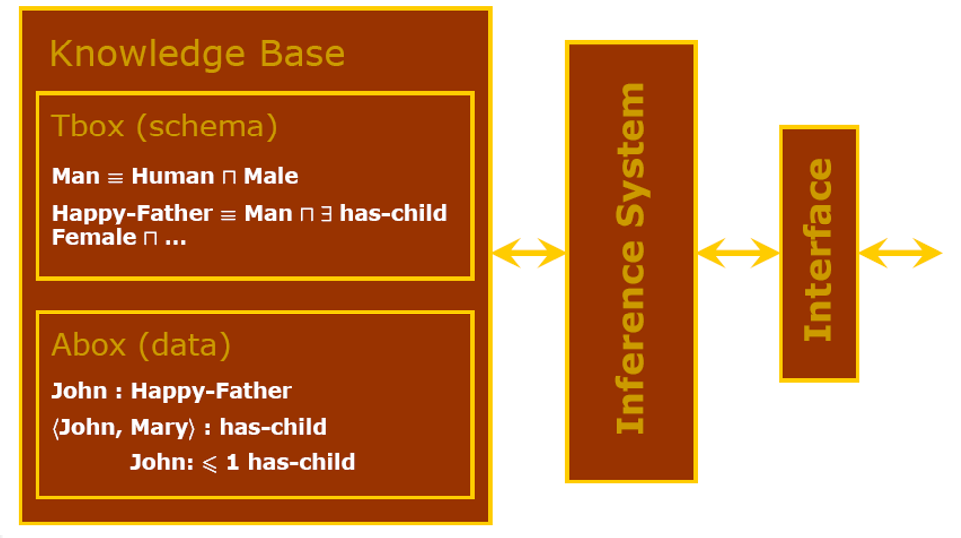
\includegraphics[scale=0.6]{IMG1.png}
\end{center}
Una classe può quindi essere definita basandosi su più classi tramite una serie di operatori logici.
La semantica dunque si definisce ricorsivamente dagli elementi più semplici ai più complessi.

\begin{tabular}{l|cl|l} \newline \newline
  Costructor & Sintassi DL & Esempio & Sintassi modale \\ \hline
  intersectionOf & $C_1 \sqcap \ldots \sqcap C_n$  & Human $\sqcap$ Male & $C_1 \wedge \ldots \wedge C_n$ \\
  unionOf & $C_1 \sqcup \ldots \sqcup C_n$ & Doctor $\sqcup$ Lawyer & $C_1 \vee \ldots \vee C_n$ \\
  complementOf & $\neg C$ & $\neg$ Male & $\neg{C}$ \\
  oneOf & $\{x_1\} \sqcup \ldots \sqcup \{x_n\}$ & $\{$ John $\} \sqcup \{$ Mary $\}$ & $x_1 \vee \ldots \vee x_n$ \\
  allVeluesFrom & $\forall P.C$ & $\forall$ hasChild.Doctor & $[P]C$ \\
  someValuesFrom & $\exists P.C$ & $\exists$ hasChild.Doctor & $(P)C$ \\
  maxCardinality & $\leq nP$ & $\leq 1$ hasChild & $[P]_n + 1$ \\
  minCardinality & $\geq nP$ & $\geq 2$ hasChild & $(P)_n$ \\
\end{tabular} \newline \newline
Dove $C$ è un concetto, $P$ una proprietà e $x$ un individuo. \newline
%\begin{center}
%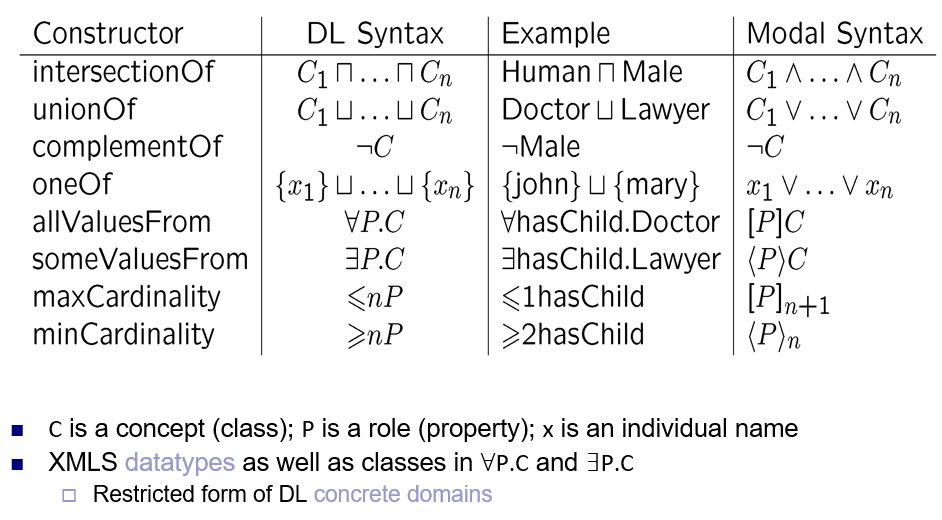
\includegraphics[scale=0.6]{IMG2.png}
%\end{center}
L'\textit{interpretazione} dei costrutti è di natura insiemistica:
\begin{center}
\begin{tabular}{rcl} \newline \newline
  $(C \sqcap D)^I$ & $=$ & $C^I \sqcap D^I$ \\
  $(C \sqcup D)^I$ & $=$ & $C^I \sqcup D^I$ \\
  $(\neg{C})^I$ & $=$ & $\Delta^I \backslash C^I$ \\
  $\{x\}^I$ & $=$ & $\{x^I\}$ \\
  $(\exists R.C)^I$ &$=$& $\{x | \exists y.<x,y> \in R^I \wedge y \in C^I\}$ \\
  $(\forall R.C)^I$ &$=$& $\{x | \forall y.(x,y) \in R^I \Rightarrow y \in C^I\}$ \\
  $(\leq R)^I$ &$=$& $\{x | \# \{y | <x,y> \in R^I\} \leq n\}$ \\
  $(\geq R)^I$ &$=$& $\{x | \# \{y | <x,y> \in R^I\} \geq n\}$ \\
  $(R^-)^I$ &$=$& $\{(x,y) | (y,x) \in R^I\}$
\end{tabular} \newline \newline
\end{center}
Dove $\Box^I$ indica l'interpretazione di $\Box$ secondo la funzione $I$. \newline
%\begin{center}
%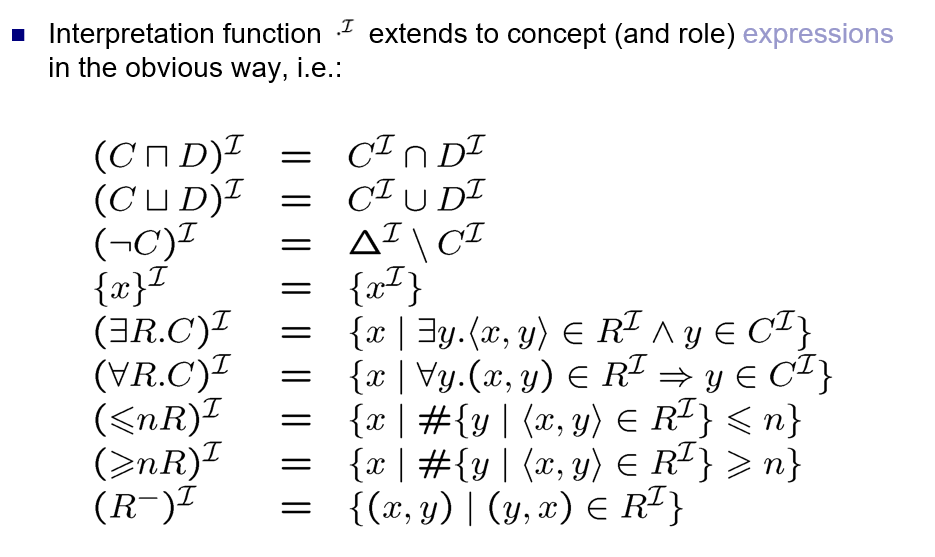
\includegraphics[scale=0.6]{IMG3.png}
%\end{center}
Gli assiomi usati in queste logiche sono estremamente semplici ma si applicano ugualmente anche a classi più complesse. Avendo infatti complicato le classi (ovvero avendo definito alcune classi come risultati di costruzioni sfruttando classi più basilari), possiamo ottenere assiomi più \textit{semplici}:
\begin{center}
  \begin{tabular}{l|c|l}
    Sintassi OWL & Sintassi DL & Esempio \\ \hline
    subClassOf & $C_1 \sqsubseteq C_2$ & Human $\sqsubseteq$ Animal $\sqcap$ Biped \\
    equivalentClass & $C_1 \equiv C_2$ & Man $\equiv$ Human $\sqcap$ Male \\
    subPropertryOf & $P_1 \sqsubseteq P_2$ & hasDaughter $\sqsubseteq$ hasChild \\
    equivalentProperty & $P_1 \equiv P_2$ & cost $\equiv$ price \\
    trnasitiveProperty & $P^+ \sqsubseteq P$ & $\text{ancestor}^+ \sqsubseteq$ ancestor
  \end{tabular}
  \begin{itemize}
  \item Sono sottintese le equivalenze FO/Modali come $DL: C \sqsubseteq D \hspace{10pt} FOL: \forall x C(x) \hspace{10pt} ML: C \rightarrow D$
  \item Si distinguono due tipi di assiomi delle TBox:
    \begin{itemize}
    \item Definizioni: $C \sqsubseteq D$ o $C \equiv D$ (dove $C$ è un concetto)
      \item GCIs (\textit{General Concept Inclusion axioms}: dove $C$ può essere complesso
    \end{itemize}
  \end{itemize}
\end{center}
% \begin{center}
% 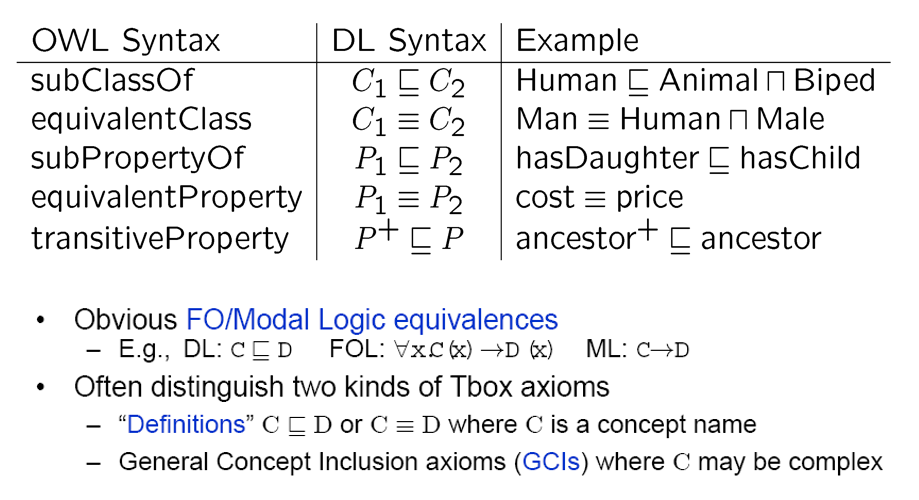
\includegraphics[scale=0.6]{IMG4.png}
% \end{center}

Possiamo dunque definire un'\textit{interpretazione} anche per gli assiomi oltre che per le classi.
L'interpretazione $I$ di un assioma soddisfa l'assioma A ($I \models A$) solamente se sono rispettate alcune regole: con una teoria logica composta da assiomi, se ne possono avere un'infinità di interpretazioni, ma ogni assioma riduce l'insieme di interpretazioni possibili, poichè ogni assioma aggiuntivo rappresenta un'ulteriore vincolo sull'ontolgia.

Un'ontologia ha esattamente questo compito: ridurre il numero di interpretazioni (riducendo così l'ambiguità) e permettere l'inferenza.
\begin{center}
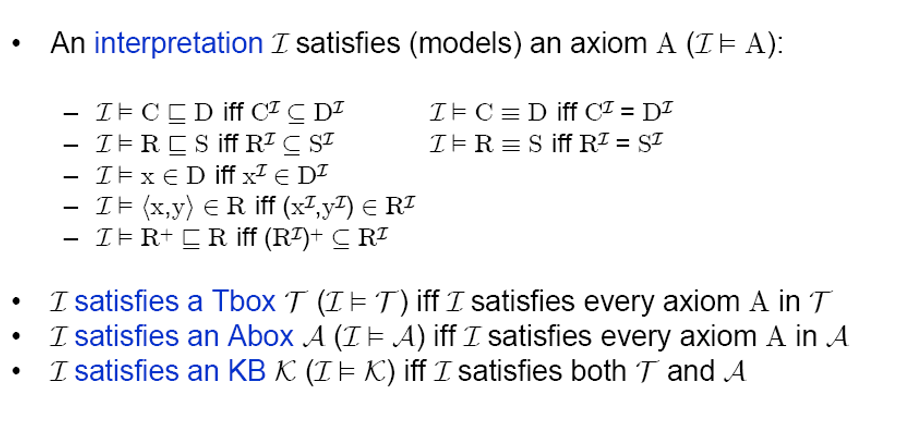
\includegraphics[scale=0.65]{IMG5.png}
\end{center}
Un concetto si dice:
\begin{itemize}
\item \textit{Soddisfacibile} se esiste almeno una sua interpretazione; 
\item \textit{Sussunto} a un altro concetto se qualsiasi interpretazione del primo concetto è sottoinsieme di un interpretazione del secondo;
\item Due concetti si dicono \textit{equivalenti} se l'interpretazione del primo concetto è sempre uguale a quella del secondo in tutte le interpretazioni della teoria, al contrario si dicono \textit{disgiunti}.
\end{itemize}
Il concetto di interpretazione in logica quindi è puramente teorico: è lo strumento matematico usato per attribuire un significato ai dati; l'inferenza permette di attribuire significati aggiuntivi indipendentemente dalla semantica iniziale.

È possibile utilizzare un \textit{reasoner} per verificare la correttezza delle relazioni.
La conoscenza ha senso solo se è \textit{soddisfacibile}: una teoria è incosistente se non ha interpretazioni che la rendono vera; caso analogo si verifica quando una classe è \textit{sussunta} all'insieme \textit{vuoto}: in tal caso non ha interpretazioni possibili.

Da un punto di vista pragmatico, con un \textit{reasoner} possiamo:
\begin{itemize}
\item Fare un check di consistenza;
\item Inferire nuove relazioni;
\item Inferire gerarchie;
\item Ereditare proprietà;
\item Inferire la classe degli individui.
\end{itemize}
In proposito ad OWL \textit{DL} occorre specificare una distinzione molto netta tra:
\begin{itemize}
\item Assunzione del \textit{mondo chiuso}, tipica dei database relazionali, per cui tutto ciò che è al di fuori del database è da ritenersi falso;
\item Assuzione del \textit{mondo aperto}, tipica di ontologie e logiche descrittive, per cui tutto ciò che è fuori \textit{potrebbe} essere vero tanto quanto ciò che è dentro.
\end{itemize}
Inoltre sempre riguardo OWL, in quanto base di conoscenza, occorre fare riferimento all'assuzione denominata \textbf{Unique Name Assumption}, che in OWL appunto non ha valore, poichè due oggetti con lo stesso nome possono indicare due cose distinte, non necessariamente essere la stessa cosa.

\subsection{Rule based reasoning}
I rules-based reasoning, a differenza dell'OWL reasoning permettono di definire delle funzioni al loro interno in grado ad esempio di effettuare ragionamenti di natura quantitativa. 

SWRL (Semantic Web Rule Language) è un linguaggio rules-based che combina OWL con RuleML, ma non è \textbf{decidibile}.
Alternativo a SWRL in questo aspetto è DLP, un linguaggio che permette di instaurare delle relazioni d'ordine per gli oggetti, come ad esempio \textit{antenato-genitore}.
RuleML (Rule Markup Language) è una famiglia di linguaggi sviluppati per esprimere sia regole \textit{forward} che \textit{backward} in XML per effettuare deduzioni ed operazioni inferenziali.


%\section{\textit{Search Engine} semantici}
\section{Search Engine semantici}
Un \textit{search engine} semantico sfrutta una base di conoscenza per effettuare delle query più mirate.
Per la gestione di pattern di architettura ci sono tre possibili approcci:
\begin{itemize}
\item \textbf{Crawling}: i dati sono memorizzati in un database locale;
\item \textbf{On-the-fly deferencing}: gli URI sono deferenziati quando il programma richiede i dati;
\item \textbf{Federated query}: ogni richiesta è delegata ad un servizio diverso.
\end{itemize}
Anche per il \textit{reasoner} ci sono strategie diverse.

%\section{\textit{Semantic Framework}}
\section{Semantic Framework}

Si usano dei framework per archiviare i dati in grafi per la facilità della gestione delle relazioni (si interroga per ottenere nuova conoscenza):
\begin{itemize}
\item \textbf{RDF4J} è un framework per Java per gestire, archiviare (in diversi modi) e interrogare documenti RDF, organizzando tramite un paradigma ad oggetti;
\item \textbf{Apache Jena} è un'api per RDF, offre un reasoner organizzando i dati ad oggetti;
\item Un \textbf{triplestore} archivia le triple e le filtra per elementi fissati ed è fatto per ricevere query SPARQL. Ci permette di fare inferenza per mezzo di reasoner o entailment ma non ha struttura interna, poichè non ha struttura per le proprietà. Alcuni esempi di triplestore sono \textit{Openlink Virtuoso}, che permette di avere più grafi e di avere quindi strutture quadruple e non triple e \textit{AllegroGraph};
\item \textbf{Property Graph} a differenza del triplestore ha una struttura interna a costo però di perdere la possibilità di effettuare inferenza. Alcuni esempi di property graph sono \textit{GraphDB8} e \textit{Neo4j}.
\end{itemize}
Tra i reasoner più conosciuti vi sono:
\begin{itemize}
\item Pellet (OWL DL);
\item Racer (OWL DL);
\item Hermit;
\item Reasoner nativi di Jena, GraphDB8 e AllegroGraph.
\end{itemize}

\newpage
\part{Problemi di matching ed integrazione semantica}
\section{Integrazione di grafi di conoscenza}
L'integrazione virtuale (l'uso di predicati \verb|sameAs| e simili) non è una funzione particolarmente scalabile con grossi database: per fare questo è necessario effettuare un'integrazione in altro modo (\textit{data integration}).
La \textit{data integration} nel caso dei grafi di conoscenza parte da una base di diversi oggetti, nel caso più semplice una \textit{source} ed un \textit{target}, che è necessario unire per aumentare il potere informativo creando un unica base di conoscenza più ampia e completa. Per effettuare con successo questa operazione è però necessario usare dei \textit{mapping}.

L'operazione di \textit{linking data} avviene a due livelli distinti:
\begin{itemize}
\item A livello di schema: effettuando un \textit{mapping} tra concetti e proprietà (anche detto \textit{ontology mapping}); \item A livello di istanze: ovvero effettuando un \textit{mappping} tra entità descrittive in sorgenti eterogenee. Ciò può avvenire tramite \textit{entity co-resolution} (\verb|sameAs|), \textit{link discovery}, \textit{instance matching} o \textit{record linkage}).
\end{itemize}
Quando si costruisce un grafo di conoscenza (soprattutto verticale, ovvero su un solo tema ma in modo approfondito), si parte innanzitutto da un'operazione di \textit{data ingestion}. 

Generalmente questa operazione avviene da fonti di dati strutturate o semi-strutturate come tabelle o database relazionali.
Si può effettuare una traduzione semantica della tabella (\textit{mapping}) per convertire una tabella in formato RDF, però facendo questo si trascurano le relazioni e le loro proprietà e non si ha controllo sugli elementi duplicati. Un tool molto usato per assolvere a questo compito di conversione da formato tabellare ad RDF è \textbf{DataGraft}.

La trasformazione da tabelle a \textit{Knowledge Graph} può presentare una serie di criticità che occorre affrontare predendo determinati accorgimenti:
\begin{itemize}
\item Normalizzare la tabella;
\item Annotare i diversi componenti della tabella con i componenti del \textit{KG}, sia a livello di schema assegnando concetti e proprietà alle colonne, sia a livello di istanze assegnando entità ai valori della tabella;
\item Si possono usare strumenti quali R2ML per annotare le tuple del database relazionale e mappandole con programmi scritti \textit{ad hoc}. Questo avviene per operazioni di \textit{mapping} particolarmente complesse. Gli strumenti di \textit{semantic table annotation and integration} tentano di stabilire quali entità esistono in un database e aiutano nella costruzione di un grafo di conoscenza;
\item Solo dopo questi accorgimenti e passaggi è possibile eseguire il \textit{mapping} finale e rappresentare il contenuto della tabella come \textit{KG}.
\end{itemize}
Un altro modo per accrescere un grafo di conoscenza è quello di processare testi (prendento informazioni dall'abstract di \url{wikidata.org}, per esempio): strutturare informazioni in formato tabellare è un processo lungo e costoso, dunque è indispensabile sfruttare tecniche di \textit{Natural Language Processing} (NLP) per estrarre informazioni direttamente da testi, tweet, abstract; tuttavia l'uso di abbreviazioni o espressioni gergali rende difficile un processo automatico del testo.
Da una parte il problema è strutturare informazioni da un testo (\textit{information extraction}), tipico caso di studio di intelligenze artificiali e semantica computazionale, mentre dall'altra è difficile rendere utile l'informazione estratta integrandola all'interno della base di conoscenza.
Gli obiettivi dell'estrazione delle informazioni sono la \textit{named entity recognition} e la \textit{relation extraction}: la prima serve per riconoscere un'entità di un testo, mentre la seconda tenta di stabilire le relazioni tra queste entità.
Per integrare le entità in un grafo di conoscenza, si effettua un'opearazione di \textit{entity linking}.

\subsection{Matching}
L'operazione di matching può risultare molto complessa a seconda del caso specifico e necessita di una serie di passaggi:
\begin{itemize}
\item Per prima cosa, occorre valutare la \textit{similarità} tra due entità appartenenti a fonti diverse tramite un opportuno indice; il problema (nei sistemi classici) tuttavia è trovare un criterio di similarità opportuno poichè a seconda del problema specifico la misuradi similarità più opportuna potrebbe variare.
\item Successivamente occorre combinare i risultati in modo ottimale: ogni indice si sofferma su un aspetto diverso del problema e devono essere combinati in modo opportuno.
Questo processo è fondamentale per interrogare diverse basi di dati con una sola query.
Di fatto quest ultimo problema è risolto tramite tecniche di apprendimento automatico (\textit{machine learning} o \textit{deep learning}), che ricavano una funzione di sintesi in modo automatico.
\item Combinati i valori, si ha comunque un problema di decisione (cosa includere nel grafo di conoscenza), introducendo un valore di soglia o tramite tecniche di ottimizzazione, o ancora tramite tecniche di apprendimento automatico.
\end{itemize}
In rarissimi casi tuttavia un algoritmo riuscirebbe a ottenere prestazioni pari a quelle umane: integrando grandi quantità di dati l'automatizzazione è necessaria ma situazioni critiche richiedono l'intervento umano.
Si deve quindi trovare un compromesso tra automatizzazione e intervento umano grazie all'\textit{interattività}, soprattutto in caso di risultato incerto. 

Oltre tutto ciò occorre anche definire che tipo di similarità stiamo ricercando, poichè ne esistono di diveri tipi:
\begin{itemize}
\item Similarità sintattica, per cui si ricerca un'uguaglianza tra due parole che hanno la stessa forma, ma questo presta il fianco alla possibilità di effettuare un matching errato assumendo che due parole uguali rappresentino sicuramente la stessa cosa;
\item Similarità lessicale, basata sui sinonimi, che però rischia di creare molta ambiguità;
\item Similarità strutturale, che tiene conto di come gli oggetti che intendiamo matchare siano inseriti nelle rispettive strutture, ma a seconda delle basi di dati potremmo trovare strutture completamente differenti e, a quel punto, questo particolare tipo di similarità provocherebbe molti problemi.
\end{itemize}
L'approccio \textit{pay as you go} tenta di integrare dando una priorità ai dati, che nel tempo saranno consolidati e modificati: così facendo si possono automatizzare dei processi, offrendo un risultato sporco, in attesa di una rifinitura umana.

%La \textit{similarità lessicale} è la prossimità tra il significato di due parole; si usano anche sistemi basati sull'analisi di dati.
%Due proprità possono anche essere simili perchè collegano entità dello stesso tipo (stesso range e stesso dominio).
%Tuttavia si hanno delle difficoltà dovute alla polisemia dei termini: proprio per questo, il problema non è trovare l'algoritmo perfetto ma trovare la combinazione migliore tra più criteri.
Si tenta di sfruttare le stesse ontologie per fonti diverse, nonostante questo non sia sempre possibile (perchè di fatto possono essere preferiti linguaggi propri anche con \textit{open data}).

\subsection{Ontology matching: \textit{Agreement Maker}}
Come già detto, l'\textit{ontology matching} è il task che ha l'obiettivo di troavare corrispondenze tra entità appartenenti ad ontologie differenti. A questo proposito \textit{Agreement Maker} è un \textit{tool} per aiutare esperti di dominio proprio nel processo di \textit{ontology matching} (ovvero matching a livello di schema): è considerato uno dei migliori esistenti a livello internazionale.

I metodi utilizzati dal software possono essere diversi:
\begin{itemize}
\item \textit{Concept based}
\item \textit{Structure based}
\item \textit{Instance based}
\end{itemize}
Si tenta quindi di costruire delle corrispondenze tra termini appartenenti a ontologie diverse: la prima si chiama \textit{source ontology} che si allinea alla \textit{target ontology}.
Mappando la \textit{source ontology} si calcola un valore di confidenza per il processo di matching; inoltre si può stabilire la cardinalità tra sorgente e obiettivo: una cardinalità \verb|1:1| stabilisce una relazione unica tra due entità, così come \verb|1:n| stabilisce un rapporto per cui ad un'entità della fonte ne corrispondono più nell'obiettivo.

In sostanza il software esegue la definizione dei matching seguendo dei passaggi precisi:
\begin{enumerate}
\item Prende in input la \textit{source ontology} e la \textit{target ontology};
\item Effettua il calcolo della misura di similarità scelta;
\item Costruisce una matrice di similarità;
\item Applica i vincoli di cardinalità;
\item Infine definisce i matching risultanti.
\end{enumerate}
\begin{center}
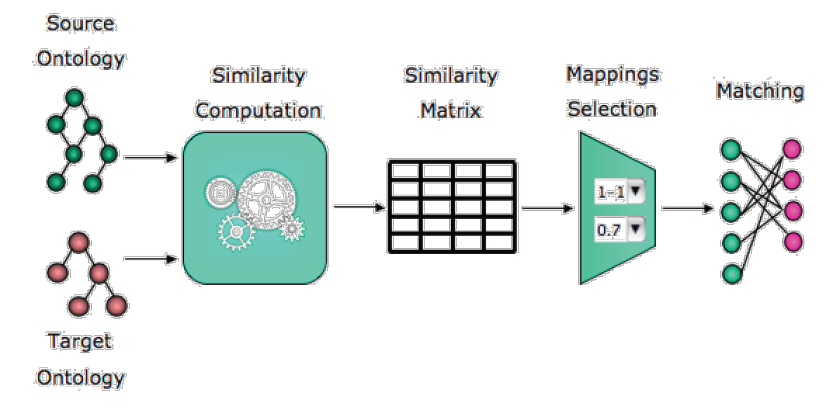
\includegraphics[scale=0.7]{IMG6.png}
\end{center}
Il software nella versione normale calcola una matrice di similarità di dimensioni $N \times M$ (dove $N$ ed $M$ sono le cardinalità delle due ontologie) usata per individuare relazioni di equivalenza.
Si effettua un \textit{match} solamente sugli elementi che superano una certa soglia.
Le dimensioni della matrice però degenerano velocemente e quindi la gestione della memoria è ardua: la versione \textit{lite} tuttavia conserva in memoria solamente i valori superiori alla soglia, così da ridurre la memoria utilizzata.

Gli indici utilizzati sono:
\begin{itemize}
\item La \textit{precision} $P = \frac{TP}{TP+FP}$ (dove $TP$ sono i valori classificati correttamente come positivi e $FP$ i valori classificati scorrettamente come positivi);
\item La \textit{recall} $R = \frac{TP}{TP+FN}$ (dove $FN$ sono i valori classificati scorrettamente come negativi);
\item La loro media armonica \textit{F-measure} $F =2 \frac{P \cdot R}{P+R}$
\end{itemize}
Queste misure sono usate in \textit{machine learning} per misurare la bontà di adattamento di un classificatore generico. 

Il processo attraverso cui Agreement Maker (come altri tool) sottopone i dati si articola su 3 livelli, che a loro volta si articolano nell'utilizzo e nella combinazione dei risultati di più matcher basati su aspetti differenti tra loro:
\begin{itemize}
\item \textbf{First layer}: concettuale
\begin{itemize}
\item BSM Base Similarity Matcher
\item PSM Parametric String-based Matcher
\item VMM Vector-based Multi-term Matcher
\end{itemize}
\item \textbf{Second layer}: strutturale
\begin{itemize}
\item DSI Descendant's Similarity Inheritance
\item SSC Sibling's Similarity Contribution
\end{itemize}
\item \textbf{Third layer}
\begin{itemize}
\item LWC Linear Weighted Combination
\end{itemize}
\end{itemize}
Con particolare riferimento al \textbf{VMM}, un testo è riassunto come insieme di termini, costruendo documenti virtuali per gli oggetti da comparare con pesi preimpostati: si calcola quindi la \textit{cosine similarity} usando le frasi come vettori:
\begin{equation*}
\cos(\theta) = \frac{A \cdot B}{\vert\vert A \vert\vert \cdot \vert\vert B \vert\vert}
\end{equation*}
Al secondo livello, prendendo in input i risultati dei matcher precedenti e basandosi sul principio che la similarità è ereditabile e può anche essere comparata tra nodi fratelli, si possono calcolare indici come il \textbf{DSI} ed il \textbf{SSC}, entrambi basati sul prendere in input i risultati del \textbf{BSM}.

L'indice $DSI \in [0; +1]$ modifica la similarità base tenendo conto della similarità dei nodi ascendenti.
\begin{equation*}
  DSI = MCP \cdot bas\_sim(C, C^*) + \frac{2(1 - MCP)}{n \cdot (n + 1)} \sum_{i=1}^n(n + 1 - i) \cdot base\_sim(parent_{C_i}, parent_{C^*_i})
\end{equation*}
Dove \textit{MCP}, il \textit{main contribution percentage}, empiricamente è un valore intorno a $0.75$ in quanto la similarità dei nodi ascendenti tende a $0.25$. \newline

L'indice SSC invece modifica la similarità base considerando la similarità tra i nodi fratelli:
\begin{equation*}
  SSC = MCP \cdot bas\_sim(C, C^*) + \frac{1-MCP}{n}\sum_{i=1}^n{\max\{base\_sim(S_i, S_1) ... base\_sim(S_i, S_m)\}}
\end{equation*}
Sia in riferimento ai valori di misure come \textit{Precision} e \textit{Recall}, che in merito a tempi di esecuzione, l'indice \textit{DSI} si dimostra spesso il migliore.

Una volta superata la fase di calcolo della similarità e di creazione della corrispondente matrice occorre passare attraverso la fase di \textit{selezione} dei mappings che prende in input:
\begin{itemize}
\item Matrice di similarità;
\item Un valore soglia definito dall'utente;
\item Una cardinalità per le corrispondenze tra source e target.
\end{itemize}
Per assolvere a questo scopo, con particolare riferimento a relazioni di cardinalità 1:1, è spesso utilizzato il sisterma \textit{greedy}: tuttavia questo massimizza solamente il match del singolo elemento e non complessivamente; si tratta di un problema di \textit{assegnamento}, risolvibile tramite metodi combinatori (\textit{Hungarian Method}, di complessità cubica) ma molto pesanti computazionalmente.
Approccio ottimale per risolvere il problema è selezionare solamente i match che superano una certa soglia e utilizzare l'algoritmo \textit{maximum matching}, che ha complessità quadratica (e quindi computazionalmente più efficiente).
Proprio per questo motivo, Agreement Maker nella sua versione Lite conserva una matrice di similarità sparsa.

Grazie a tecniche di \textit{machine learning} si possono calcolare soglie, combinazioni lineari tra i \textit{matcher} o ancora costruire \textit{matcher} nuovi (nonostante sia richiesta una gran quantità di esempi).

Un approccio molto diffuso, alternativo alla semplice combinazione dei risultati dei diversi matcher, per rendere il matching più affidabile e snello è quello della combinazione dei risultati dei matcher basata però sulla qualità del matching stesso. Un esempio di misura di qualità, se è noto, è un \textit{gold standard} (ovvero un esempio i cui risultati sono già noti). Molto raramente si presenta questa possibilità ed è quindi necessario ricorrere a misure di qualità differenti:
\begin{itemize}
\item A livello globale abbiamo più che delle misure, delle vere e proprie euristiche: quella di conservazione della distanza che si basa sul fatto che un match \textit{F} tra due concetti in due ontologie non dovrebbe distorcere la distanza che c'è tra i concetti stessi e quella di conservazione dell'ordine che afferma la stessa cosa ma in merito all'ordine che i concetti possiedono all'interno delle rispettive ontologie;
\item A livello locale con il calcolo di una vera e propria misura di confidenza.
\end{itemize}
Un buon \textit{matcher} dovrebbe dare un'alta affidabilità a pochi collegamenti, e dovrebbe restituire un'affidabilità nulla in caso di elementi non compresi nell'ontologia.
Inoltre, può capitare che certi concetti siano identificati meglio di altri: si calcola così il livello di confidenza locale
\begin{equation*}
  LC_M(c) = \frac{\sum_{c' \in m_M(c)}sim_M(c, c')}{|m_M(c)|} - \frac{\sum_{c' \in (T - m_M(c))}sim_M(c, c')}{|T - m_M(c)|}
\end{equation*}
Il livello di confidenza così calcolato a livello locale ci permette di definire dei pesi basati sulla qualità dei matching dei singoli matcher e, una volta definiti i pesi, di utilizzarli per combinare i risultati dei diversi matcher in una vera e propria media pesata \textit{LWC}. A questo punto, sulla scia di quanto detto in precedenza, si può procedere a calcolare i diversi indici già noti, come il \textit{DSI}. In sostanza l'approccio basato sulla qualità ha lo scopo primario di dare un peso diverso all'apporto di ogni matcher sul risultato finale basandosi sulla qualità del matcher misurata \textit{localmente}.
\newline
\newline
Quanto detto finora vale soprattutto per il matching e la valutazione di ontologie reali molto grandi ma esistono tutta una serie di task analoghi che presentano ancora molte criticità e sfide:
\begin{itemize}
\item Per le ontologie \textit{linked open data} le cose sono più complesse;
\item Cross-lingual ontology matching;
\item Metodi di matching interattivi;
\item Semantic table annotation.
\end{itemize} 
%ho aggiunto quest'ultima parte anche se il professore non sembrava particolarmente interessato ad approfondirla, ma magari più avanti la riprenderà.

\subsection{\textit{Instance matching}}
È un problema relativo alle basi di dati: si tratta di effettuare un \textit{record linkage} (se fatto su due dataset diversi) o \textit{deduplication} (se fatto sullo stesso dataset).
% Batini, Information Qualtiy, Springer
Lo stesso oggetto del mondo reale può corrispondere a più oggetti in un database, e servono tecniche per identificare le corrispondenze; inoltre i valori possono essere comunque diversi; tra due database diversi persino l'identificativo può non corrispondere, complicando il processo.
Ci possono essere persino errori voluti: in piattaforme di compravendita, il criterio più usato per ordinare è per prezzo crescente, quindi venditori di accessori possono dichiarare di vendere il prodotto per salire più in alto nella lista.

La tecnica più diffusa di matching prevede che siano dati per corretti link con valore superiore ad una certa soglia, e incerti se superiori ad un'altra soglia più bassa (tecnica della doppia soglia), che saranno poi confermati dall'utente.

Le tecniche si dividono in varie categorie.

\paragraph{Empirico.}
È un sistema che calcola la similitudine tra due tuple considerando solo la prossimità ortografica (tenendo anche conto della distanza dei tasti sulla tastiera).
È usato per migliorare il matching dopo l'uso di altre tecniche.

\paragraph{Probabilistico.}
Usa delle tecniche probabilistiche per calcolare la distanza tra due tuple.

% manca uno
% \paragraph{}

\paragraph{Misti.}
Mischia le ultime due tecniche per effettuare un match migliore.
\newline

Le dimensioni delle ontologie possono essere problematiche dato che le comparazioni da effettuare sono $n_1 \times n_2$, il prodotto cartesiano tra i due dataset.
Si usano quindi tecniche di \textit{blocking} per ridurre il numero di comparazioni e quindi lo spazio della ricerca.
Anche in database a grafo e rappresentazioni RDF si hanno problemi simili con delle differenze minime.
Ridotto lo spazio di ricerca, si applica un modello che distingua tra \textit{match}, \textit{possible match} o \textit{not match}.

L'approccio probabilistico usa tecniche di \textit{machine learning} per identificare i \textit{match}, generando un algoritmo proprio.
L'algoritmo sceglie una funzione di distanza (o una combinazione di più funzioni) e valori soglia in modo automatico.

\paragraph{\textit{Preprocessing}.}
Per prima cosa i dati devono essere normalizzati eliminando variazioni sintattiche o armonizzando gli standard.
Inoltre si tenta già di filtrare (tramite \textit{parsing} o \textit{machine learning}) i dati in modo da estrarre entità dal dato.

\paragraph{\textit{Blocking}.}
Per ridurre il numero di comparazioni da effettuare, si cerca una chiave su cui ordinare i record in entrambe le tabelle; si usa quindi una finestra mobile per cercare collegamenti in posizioni simili.
La complessità passa da $O(n^2)$ a $O(\frac{m^2n}{m})$ (dove $m$ è la dimensione della finestra).

\paragraph{Distanza.}
La distanza tra due tuple è l'elemento su cui è effettuata l'indagine statistica: minore è la distanza, maggiore è la percentuale di \textit{match}; altro punto cruciale è la scelta della soglia.
Il valore deve dare delle buone prestazioni ma allo stesso tempo ridurre il numero di richieste fatte all'utente.
Si considerano analoghe due tuple con distanza minore della soglia.
\newline

Il processo è effettuato su un campione di dati di una certa dimensione; per migliorare ulteriormente la qualità dell'algoritmo si possono anche usare tecniche di \textit{active learning} usando solamente osservazioni critiche per costruire il campione.

\subsection{\textit{Pay as you go}}
Si usa l'approccio \textit{pay as you go} per aggiungere osservazioni da analizzare in modo automatico e quindi migliorare la classificazione in momenti successivi alla pubblicazione dell'algoritmo.

\subsection{Gestione dei conflitti con la textit{data fusion}}
La gestione dei conflitti può essere fatta rimuovendo il match, aggiungendo metadati per far sì che la scelta rimanga all'utente o impostare una gerarchia tra le osservazioni (come far prevalere la più recente).
Questi tuttavia non sono metodi finali di risoluzione ma solamente sistemi di ausilio.

\section{Analisi del testo}
Si usano tecniche di analisi testuale per processare i testi:

\paragraph{\textit{Stop words}.}
Si eliminano le parole più diffuse che non alterano il senso principale della frase (nell'analisi), come congiunzioni o articoli.

\paragraph{Tokenizzazione.}
Si regolarizzano i nomi eliminando la punteggiatura.

\paragraph{Lemmatizzazione.}
Si riconduce una parola alla sua radice, in modo da estrapolare più facilmente il significato; tuttavia si rischia di sottovalutare l'ambiguità sintattica.

\paragraph{Streming.}
TO DO.
% to do
\newline

Si usano quindi misure di similarità sulla tupla processata per eseguire i match.
Questi comparano i singoli elementi della tupla, quindi il risultato delle funzioni sopracitate.
La similarità deve essere $sim(x, y) = 1$ in caso di corrispondenza perfetta.

Si parla anche di \textit{metrica} di dimensionalità, se sono rispettate certe caratteristiche:
\begin{align*}
  dist(x, x) &= 0 \\
  dist(x, y) &\ge 0 \\
  dist(x, y) &= dist(y, x) \\
  dist(x, y) &\le dist(x, z) + dist(y, x)
\end{align*}
Le ultime due proprietà tuttavia non sono sempre rispettate da tutti gli indici.

Esiste una funzione di \textit{edit distance} chiamata Levenshtein, dove ogni modifica (inserimento, cancellazione o sostituzione di caratteri) che deve essere apportata per passare da una stringa $v_1$ a una stringa $v_2$: non misura una distanza ma informa quanto il primo valore è accurato rispetto al secondo.
Tuttavia la sostituzione in caso di errori di battitura è più importante di sostituzioni casuali, e l'inserimento di spazi o altri segni di punteggiatura è eseguito in modo casuale, inoltre la modifica di cifre latine è particolarmente significativo; sono quindi calcolati pesi per le singole sostituzioni, eseguiti in modo automatico.

Altra tecnica di analisi è processare le stringhe in sottostringhe di lunghezza definita ($n$-grammi): si calcola poi una distanza considerando le tuple di $n$-grammi; questo indice è robusto rispetto agli errori di battitura ma poco rispetto alle sostituzioni (al contrario dell'indice di Jaccard).

\section{Grafo di vicinato}
Si considera \textit{grafo di vicinato} il sottografo comprendente gli elementi raggiungibili in $h$ passi da un nodo $i$.
Si comparano i grafi grazie a misure di similarità su grafi, che però sono costose: si preferisce stabilire uno spazio di \textit{features} di dimensione pari al numero di entità nel grafo, così che ogni entità abbia un suo peso.
Così si può attribuire un peso proporzionale alla distanza o al numero di relazioni che un'entità ha con le altre.

\section{\textit{Matching cross language}}
Si possono cercare match tra più lingue diverse rappresentando ogni parola come un vettore di concetti pesato.
Si cerca quindi un sistema di disambiguazione leggera: si calcola il vettore centroide (ovvero medio) tra le due stringhe per calcolare la distanza.
Questo sistema funziona bene per testi brevi, ma la complessità degenera con la lunghezza del documento.

\section{Estrazione di informazioni in formato tabellare}
Il web è pieno di dati in formato tabellare difficili da elaborare in modo adeguato.
% se questa mi tira ancora la coda addosso gliela taglio
Le problematiche riguardano la struttura delle tabelle (che possono anche non seguire il modello relazionale) o il significato semantico dell'\textit{header}.
Spesso le tabelle processate sono il risultato di \textit{denormalizzazione} dei dati, ovvero in cui sono esplicitate relazioni interne ai dati.
Si possono usare tecniche automatiche o \textit{tools} che processano le tabelle in modo automatico.

Generalmente la prima riga (l'\textit{header}) contiene indicazioni sulla struttura della tabella; inoltre si può ipotizzare una colonna implicita con informazioni aggiuntive ricavabili solamente dal contesto.
Una tabella è processata costruendo un grafo \textit{a stella} il cui nodo principale è il \textit{soggetto} e i restanti sono le relazioni; il soggetto si intende a livello semantico, e risulta essere un oggetto in RDF (deve però essere un URI); le altre colonne sono annotate come proprietà.
Si possono definire classi proprie, o usare una o più ontologie per integrare i dati, determinando vari livelli di approfondimento.
Così facendo si mappa lo schema per ottenere un grafo di conoscenza.

Esistono modelli più complicati, per adattare i dati allo schema (eseguendo anche operazioni di \textit{preprocessing}), come OpenRefine, sviluppato da Google e poi reso \textit{open source}.
Altri strumenti ipotizzano strutture dai dati tabellari grazie ad algoritmi di \textit{machine learning} per automatizzare il processo.
ASIA (\textit{Assisted Semantic Interpretation and Annotation of tabular data}) aiuta a trasformare dati tabellari in grafi RDF e permette inoltre di aggiungere annotazioni a livello di schema o di singola istanza.
Applica inoltre tecniche di \textit{record linkage} per integrare dati tabellari in un grafo RDF già esistente.

\section{Estrazione di informazioni in formato non strutturato}
Per \textit{formato non strutturato} si intendono testi in linguaggio naturale e documenti audiovisivi (audio, video o immagini).

Per i testi in linguaggio naturale, esistono plugin\footnote{Clear Forest Gnosis Mozilla Plugin.} (NER, \textit{Named Entity Recognition}) che estraggono informazioni in automatico da pagine web, identificando la loro natura.
Inoltre si possono costruire modelli di estrazione di relazioni, che collegano oggetti appartenenti allo stesso documento identificando il rapporto che le lega.
Generalmente queste due tecniche sono usate assieme per analizzare un testo.

Esistono tecniche di \textit{natural language processing} che effettuano \textit{deep parsing}, ovvero l'analisi grammaticale del testo e la successiva analisi logica, usano \textit{machine learning} o sfruttano vocabolari interni.
Gli algoritmi statistici (\textit{deep learning}) hanno suscitato forti dibattiti in ambito accademico dato che non sono interpretabili in nessun modo dagli esperti di dominio.
Spesso però manca la quantità sufficiente di dati per poter eseguire tecniche statistiche.

Le tecniche per l'analisi del testo cambiano in base alla qualità del testo stesso (in base al registro utilizzato); però nessuna tecnica ha una precisione perfetta.

\section{Estrazione di relazioni}
I metodi basati sul \textit{machine learning} non sono i migliori per gestire le relazioni (l'unico approccio che offre risultati soddisfacenti è il \textit{never ending learning}).
L'approccio più competitivo usa delle regole linguistiche sulle triple RDF per trovare le relazioni tra le entità; tuttavia sono algoritmi estremamente costosi da implementare e come licenza software.

\subsection{\textit{Name Identity Extraction} da Twitter}
% cogito
I \textit{social media} sono strumenti per estrarre informazioni non ufficiali; si hanno informazioni aggiornate e quindi nuova conoscenza.
L'estrazione di informazioni da Twitter è però difficile a causa della presenza di \textit{hashtag} che non rispettano le regole grammaticali pur rappresentando entità.
Delle entità si deve determinare il tipo (a causa della polisemia), discriminando anche se si tratta di entità reali o di finzione: si tratta di risolvere le disambuiguità.

Le disambuiguità possono essere risolte a partire dal testo, ma in alcuni casi è necessario avere una conoscenza di dominio.
Per ogni parola si possono avere più candidati: quella ritenuta corretta massimizza la somiglianza tra i membri della lista.
Il \textit{bottleneck} è il riconoscimento delle entità all'interno del testo.

In Twine, si effettua una prima fase di NER (con un algoritmo \textit{black box}) che estrae le \textit{surface form}, ovvero la stringa di caratteri che denota la menzione dell'entità del tweet, su cui è poi effettuato un match con distanza coseno; si considerano quindi i candidati migliori per poi analizzare dati di appoggio (si estrae l'\textit{abstract} per confrontarlo con il testo del tweet) ottenendo dei punteggi.
Ordinati i candidati per punteggio, si tentano dei collegamenti tra le entità.
Il \textit{Knowladge score} è calcolato come:
\begin{equation*}
  KB(e_j, c_k) = \alpha \cdot lex(e_j, I_{c_k}) + (1 - \alpha) \cdot cov(e_j, c_k)
\end{equation*}
che considera la similarità lessicale ($lex$) tra le entità e la \textit{coverage} ($cov$), basata sulla coerenza e sulla popolarità degli elementi: più un'entità è popolare, più probabile sarà il match.
I componenti sono combinati linearmente con un parametro $\alpha$ con valore che ottimizza le prestazioni.
L'indice $lex$ non è normalizzato in $[0;+1]$ e non può essere normalizzato.
\begin{align*}
  lex(e_j, I_{c_j}) &= les(e_j, I_{c_j}) + W_D \frac{JW(e_j, I_{c_j})}{W_D + 1} \\
  JW(e_j, I_{c_j}) &= Jarov(e_j, I_{c_j}) + \frac{P^\prime}{10}(1 - Jarov(e_j, I_{c_j}))
\end{align*}
La \textit{jaro distance} è una misura di similarità (compresa in $[0; +1]$) dipendente dalla lunghezza di un prefisso comune a due stringhe.
Si considera valido il match se la distanza non supera una certa soglia ($\frac{1}{2}\max(|x|, |y|) - 1$).
Si considera inoltre il numero di trasposizioni $t$, ovvero i caratteri che non sono nella stessa posizione ma sono presenti in entrambe le stringhe.
La formula quindi è:
\begin{equation*}
  sim_{jaro} = \frac{1}{3}(\frac{m}{|x|} + \frac{m}{|y|} + \frac{m-t}{m}) \in [0; +1]
\end{equation*}
Questa tecnica è usata per trovare corrispondenze tra tutte le permutazioni di nome-cognome di una persona e una stringa.

La similarità di \textit{coverage} è definita come:
\begin{equation*}
  cov(e_j, I_{c_k}) = cos(e_j, a_{c_k}) + R(c_k)
\end{equation*}
dove $R(c_k)$ è il \textit{page rank} (ovvero la popolarità) della pagina twitter su cui è effettuato il match: non è però una misura normalizzata.

L'algoritmo di disambiguazione non è particolarmente lento; tuttavia il sistema di \textit{name identity recognition} (effettuato tramite apprendimento automatico) è pesante; inoltre questi algoritmi sono allenati su testi vecchi ma il linguaggio dei social network è in continua evoluzione e quindi le prestazioni effettive sono minori di quelle attese.

Si usa quindi un altro algoritmo di apprendimento (LearningToLink) che stabilisce quando effettuare il link tra elemento ed entità.
L'algoritmo quindi è usato solamente per effettuare l'ottimizzazione: il \textit{machine learning} è fondamentale solamente in questa fase.

TWINE si basa su kafka per ottenere informazioni in tempo reale e MongoDB per archiviare i dati; ma dalla versione 2 l'architettura è diventata più facile da scalare.

\section{Visualizzazione di basi di dati}
Nonostante la grande quantità di dati disponibili grazie ai \textit{linked open data}, questi non sono sufficienti a completare tutte le operazioni.
Prima di effettuare una query, si effettua una ricerca esplorativa, per ottenere informazioni aggiuntive sul dominio; quindi si tenta di ridurre l'incertezza del processo decisionale con interrogazioni mirate e raffinate.
La visualizzazione è di aiuto in fase esplorativa ma l'occhio umano non riesce a distinguere grosse quantità di informazioni.
Si astrae quindi l'informazione riducendo la scala, e visualizzando solamente riassunti semplici di informazioni complesse.
% wikigalaxy (https://wiki.polyfra.me)
I \textit{linked data} non sono indicizzati per argomento: nonostante l'ontologia sia pubblica, non sempre questa coincide con lo schema (e non sempre sono accoppiati coi dati, essendo più prescrittivo che descrittivo).

\subsection{ABSTAT}
Si tratta di un software\footnote{Disponibile su \url{abstat.disco.unimib.it}.} di \textit{data profiling} (l'operazione che tenta di estrapolare il contenuto di un dataset) estraendo dalle triple da \url{dbpedia.org} con cardinalità e altre informazioni.

\newpage
\part{Sistemi di raccomandazione}
Un \textit{sistema di raccomandazione} tenta di suggerire ad un utente degli oggetti simili a quelli da lui preferiti.
Il concetto di \textit{rilevanza} è più rilassato di quello di similarità: sono delle relazioni empiriche che collegano più entità.

\newpage
\part{Esercitazioni}

\section{SPARQL}
Si interroga \url{https://dbpedia.org} per ottenere una lista di vulcani:
\begin{lstlisting}[language=sparql]
PREFIX rdf: <http://www.w3.org/1999/02/22-rdf-syntax-ns#>
PREFIX dbo: <http://dbpedia.org/ontology/>

SELECT distinct ?v
  FROM <http://dbpedia.org>
 WHERE {
         ?v rdf:type dbo:Volcano .
       }
 LIMIT 100
\end{lstlisting}
I prefissi si aggiungono inserendo l'url tra simboli \verb|<| e \verb|>|.
\verb|rdf:type| può essere sostituito da una \verb|a|:
\begin{lstlisting}[language=sparql]
?v a dbo:Volcano .
\end{lstlisting}

Una query SPARQL è strutturata specificando:
\begin{itemize}
  \item prefissi
  \item tipo di query
  \item (fonte)
  \item (filtri)
  \item eventuali altre clausole
\end{itemize}
Le specifiche SPARQL possono essere ottenute all'indirizzo \url{https://www.w3.org/TR/rdf-sparql-query/}

\subsection*{Esercizio 1}
Si tenta di trovare il numero di dipendenti Google dalla pagina \url{http://dbpedia.org/page/Google}:
\begin{lstlisting}[language=sparql]
PREFIX res: <http://dbpedia.org/resource/>
PREFIX dbo: <http://dbpedia.org/ontology/>

SELECT ?num
  FROM <http://dbpedia.org>
 WHERE {
         res:Google dbo:numberOfEmployees ?num .
       }

# o piu` semplicemente:
SELECT ?num
  FROM <http://dbpedia.org>
 WHERE {
         dbr:Google dbo:numberOfEmployees ?num .
       }
\end{lstlisting}

\subsection*{Esercizio 2}
Si cerca di ottenere una lista di trombettisti leader di band:
\begin{lstlisting}[language=sparql]
SELECT ?person
 WHERE {
       # soggetto   proprieta`      oggetto
         ?person    dbo:instrument  dbr:Trumpet .
         ?person    dbo:occupation  dbr:Bandleader .
       }
\end{lstlisting}

\subsection*{Esercizio 3}
Si cercano i Paesi con più di due grotte:
\begin{lstlisting}[language=sparql]
  SELECT ?country
   WHERE {
           ?cave     rdf:type      dbo:Cave .
           ?cave     dbo:location  ?country .
           ?country  rdf:type      dbo:Country .
         }
GROUP BY ?country
  HAVING (COUNT(?cave) > 2)
\end{lstlisting}

\subsection*{Esercizio 4}
Si vogliono trovare tutti i software sviluppati da società californiane.
\begin{lstlisting}[language=sparql]
SELECT DISTINCT ?software
 WHERE {
         ?company rdf:type dbo:Organisation .
         {           # dbpedia validata
           ?software dbo:developer ?company .
         } UNION {   # dbpedia da validare
           ?software dbp:developer ?company .
         }
         ?software rdf:type dbo:Software .
         ?company dbo:foundationPlace dbr:California .
       }
\end{lstlisting}

\subsection*{Esercizio 5}
Verificare se Natalie Portman è nata negli Stati Uniti:
\begin{lstlisting}[language=sparql]
  ASK
WHERE {
        dbr:Natalie_Portman dbo:birthPlace ?city .
        ?city dbo:Country dbr:United_States .
      }
\end{lstlisting}

\subsection*{Esercizio 6}
Verificare se Roma è la capitale d'Italia:
\begin{lstlisting}[language=sparql]
  ASK 
WHERE {
        dbr:Italy dbo:capital dbr:Rome .
      }
\end{lstlisting}

\subsection*{Esercizio 7}
Verificare se è disponibile la data di nascita di Elizabeth Taylor.
\begin{lstlisting}[language=sparql]
  ASK
WHERE {
        dbr:Elizabeth_Taylor dbo:birthDate ?_ .
      }
\end{lstlisting}

\subsection*{Esercizio 8}
Verificare se Milano è in Germania.
\begin{lstlisting}[language=sparql]
  ASK
WHERE {
        dbr:Germany dbo:city dbr:Miland .
      }
\end{lstlisting}

\subsection*{Esercizio 9}
Verificare se Michelle Obama è sposata con Barack Obama.
\begin{lstlisting}[language=sparql]
  ASK
WHERE {
        dbr:Michelle_Obama dbo:spouse dbr:Barack_Obama .
      }
\end{lstlisting}

\subsection*{Esercizio 10}
Si cercano i giocatori di Football americano che pesano più di 100kg.
\begin{lstlisting}[language=sparql]
CONSTRUCT {
            ?x rdf:type dbo:AmericanFootballPlayer .
          }
    WHERE {
            ?x dbo:weight ?kg .
            FILTER(?kg > 1000000000)
          }
\end{lstlisting}


\section{Protégé}
Progetto \textit{Open Source} per gestire ontologie, permette di caricare direttamente l'ontologia di \url{dbpedia.org} o di \url{schema.org}.
DBPedia usa più di $400$ classi, usandone anche di \textit{sporche} (ovvero ripetute o poco utili).
Usando il \textit{reasoner}, sono evidenziate le incongruenze (ovvero classi inconsistenti), che non possono avere dunque istanze.

\subsection*{Costruzione di un'ontologia}
Si costruisce una semplice ontologia per la costruzione di un semplice domino geografico.
\begin{verbatim}
                  City  <  Region  <  Country  <  Continent
\end{verbatim}
In Protégé, si definisce una nuova ontologia con \verb|File > New| e inserendo poi sottoclassi di \verb|owl:Thing|.
Popolata l'ontologia con delle istanze arbitrarie, si definiscono le proprietà.
Si cerca di ridurre al minimo il numero di relazioni (si ha un'intuizione della definizione di contenimento), ma non è possibile tentando di ridurre al minimo le classi.
Nel menù \verb|Object properties| è possibile definire nuove proprietà e definire dominio e immagine; si attribuiscono poi le proprietà alle istanze andando su \verb|Entities > Individuals| e cliccando su \verb|Object properties assertions| (a destra).

\section{\textit{Ontology matching}}
Si tenta di fare prima dei \textit{match} a mano tramite un'analisi esplorativa, eliminando entità troppo specifiche e selezionando le corrispondenti.
Questo approccio è estremamente lento e dispendioso, per cui si tenta di automatizzarlo.
Si introducono degli operatori di \textit{matching} per indicare il rapporto tra le relazioni: \newline
\begin{center}
\begin{tabular}{cl}
  $a = b$ & $a$ corrisponde a $b$ \\
  $a \leq b$ & $a$ è più specifico di $b$ \\
  $a \geq b$ & $a$ è meno specifico di $b$
\end{tabular}
\end{center}

Si indica con $\Box^*$ se la relazione non è certa ma solamente ipotizzata.
In SKOS sono presenti tutte le relazioni, con proprietà di transitività e associatività.
\end{document}